\documentclass{beamer}

\usepackage{Haust2017glærur}

\title{Stærðfræðimynstur í tölvunarfræði}
\subtitle{Vika 10, fyrri fyrirlestur}

\begin{document}

\begin{frame}
\titlepage
\end{frame}


\section{Net}

\begin{frame}{Í síðasta tíma}
    \begin{itemize}
     \item Lausnir á rakningarvenslum
     \item Deila-og-drottna reiknirit og tímaflækjugreining
    \end{itemize}
\end{frame}

\begin{frame}{Net}
Lítum á lauslega skilgreiningu á óstefndu neti:

\begin{tcolorbox}[title=Net]
Net (e. \emph{graph}) $G = (V, E)$ samanstendur af tveimur mengjum, $V$, ekki-tómu mengi hnúta (e. \emph{vertices} eða \emph{nodes}) og $E$, mengi leggja (e. \emph{edges}). Hver leggur er tengdur við einn eða tvo hnúta, sem eru endahnútar (e. \emph{endpoints}) leggsins.
\end{tcolorbox}
\end{frame}

\begin{frame}{Dæmi}
\begin{center}
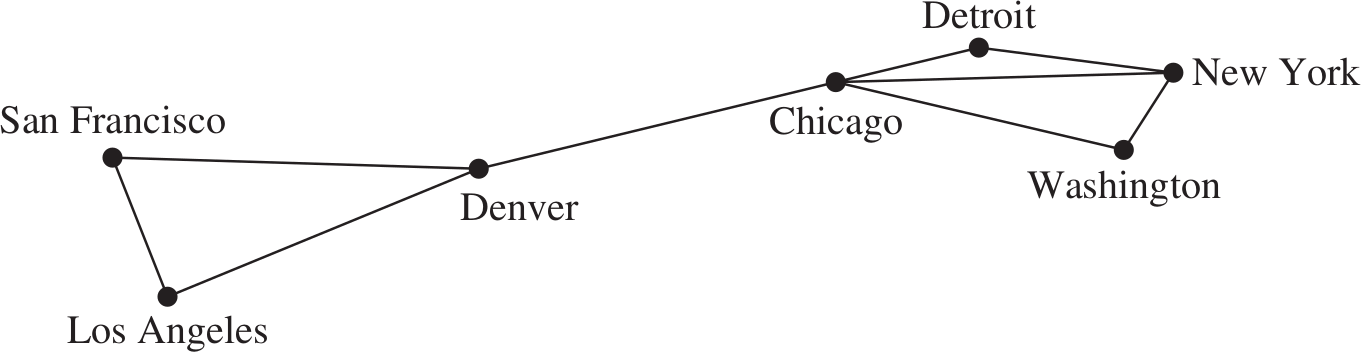
\includegraphics[width=\textwidth]{computer-network}

Einfalt net
\end{center}
\end{frame}

\begin{frame}{Um skilgreiningu}
\begin{itemize}
 \item Venjulega tölum við um endanleg net (e. \emph{finite graph}), sem hafa endanleg hnúta- og leggjamengi
 \begin{itemize}
  \item Einnig má skilgreina óendanleg net (e. \emph{infinite graph}), þar sem a.m.k. annað mengjanna er óendanlegt
 \end{itemize}
 \item Bókin gerir ekki mikið úr muninum á einföldum netum, fjölnetum og netum með lykkjum
 \begin{itemize}
  \item Í einföldu neti (e. \emph{simple graph}) tengja engir tveir leggir sömu tvo hnúta
  \item Í fjölneti (e. \emph{multigraph}) mega margir leggir liggja á milli sömu hnúta
  \item Lykkja (e. \emph{loop}) er leggur sem tengdur er við einn hnút, lykkjur geta verið bannaðar eða leyfðar
  \begin{itemize}
   \item Net með lykkjum: pseudograph?
  \end{itemize}
  \item Tökum fram hvað við eigum við þegar það skiptir máli
 \end{itemize}
\end{itemize}
\end{frame}

\begin{frame}{Dæmi}
\begin{center}
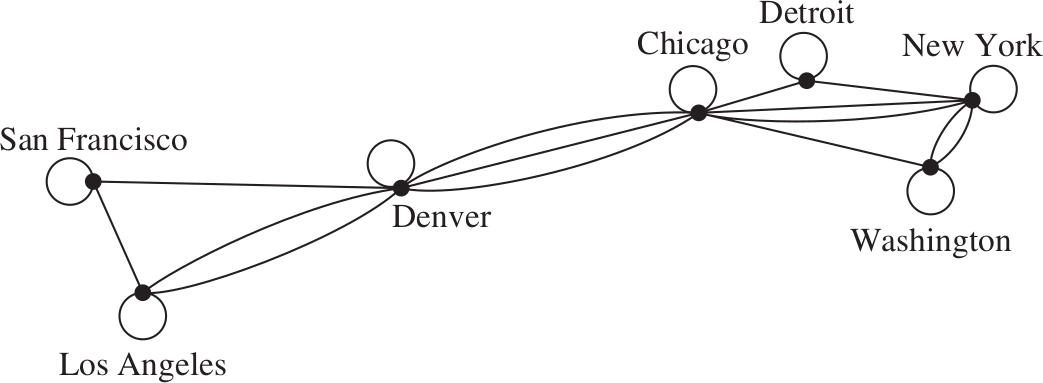
\includegraphics[width=\textwidth]{computer-network-loops}

Net með lykkjum
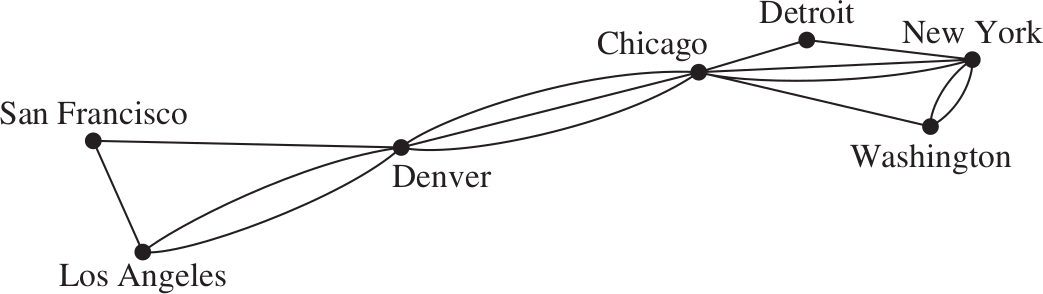
\includegraphics[width=\textwidth]{computer-network-multiple}

Fjölnet
\end{center}
\end{frame}

\begin{frame}{Stefnt net}
Rifjum upp skilgreiningu á stefndu neti:
\begin{tcolorbox}[title=Stefnt net]
Stefnt net (e. \emph{directed graph}) samanstendur af mengi $V$ af hnútum og mengi $E$ af röðuðum pörum af hnútum í $V$ sem nefnast stefndir leggir (e. \emph{directed edges}). Í leggnum $(a, b)$ er fyrri hnúturinn upphafshnútur (e. \emph{initial vertex}) og seinni hnúturinn lokahnútur (e. \emph{terminal vertex}).
\end{tcolorbox}

Getum lýst einföldum stefndum netum, stefndum fjölnetum og stefndum lykkjum á svipaðan hátt og við gerðum fyrir óstefndu netin.

Stefndir leggir eru líka kallaðir örvaleggir.
\end{frame}

\begin{frame}{Hugtakanotkun í bók}
\begin{quotation}
We will sometimes use the term graph as a general term to describe graphs with directed or undirected edges
(or both), with or without loops, and with or without multiple edges. At other times, when the
context is clear, we will use the term graph to refer only to undirected graphs.
\end{quotation} - Rosen

\end{frame}

\section{Hagnýting neta}

\begin{frame}{Hagnýting neta}
\begin{itemize}
 \item Við getum notað net til að setja fram hinar ótrúlegustu upplýsingar
 \begin{itemize}
  \item Látum þá hvern hnút tákna ákveðið fyrirbrigði og hvern legg einhvers konar samband þeirra á milli
 \end{itemize}
 \item Munum sjá reiknirit sem vinna á netum til að leysa ýmsar gerðir vandamála
\end{itemize}
\end{frame}

\begin{frame}{Samfélagsnet}
Virkar, þverfaglegar rannsóknir fara fram á netum sem tákna tengsl fólks
\begin{center}
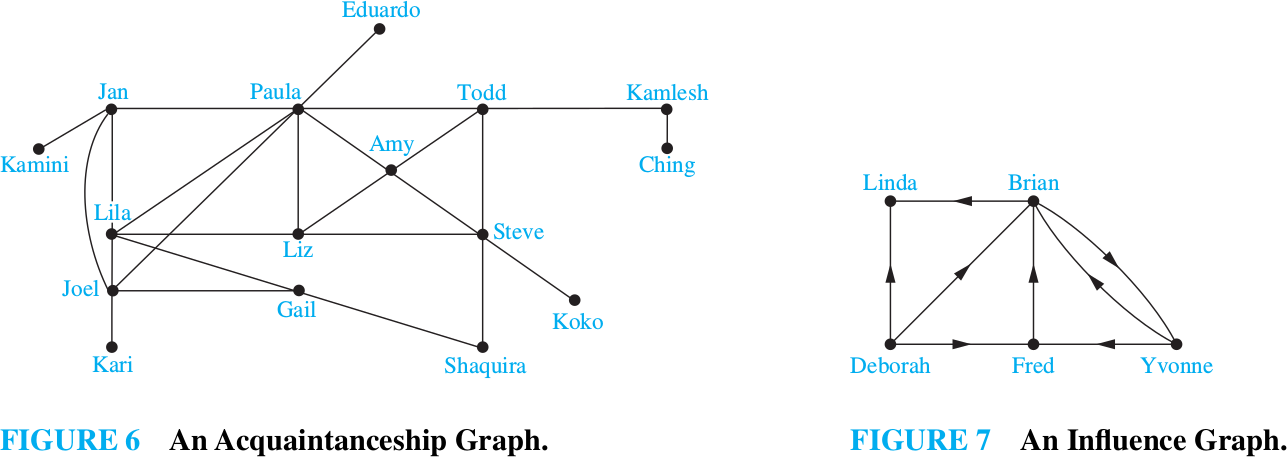
\includegraphics[width=\textwidth]{social-graphs}
\end{center}
Gæti táknað vináttu, áhrif, samstarf\ldots
\end{frame}

\begin{frame}{Netkerfi}
\begin{itemize}
 \item Borðliggjandi er að láta net tákna alls kyns samskipta- og netkerfi
 \begin{itemize}
  \item Kortleggjum símtöl
  \begin{itemize}
   \item Táknum símanúmer með hnútum, setjum legg þeirra á milli hafi þau talað saman
  \end{itemize}
  \item Kortleggjum veraldarvefinn
  \begin{itemize}
   \item Táknum heimasíður með hnútum og setjum örvalegg þeirra á milli ef ein síðan er með tengil yfir á hina
  \end{itemize}
 \end{itemize}
\end{itemize}
\end{frame}

\begin{frame}{Internetið}
\begin{columns}
\column{0.3\textwidth}
Netaframsetning (hluta?) internetsins, af wikimedia
\column{0.7\textwidth}
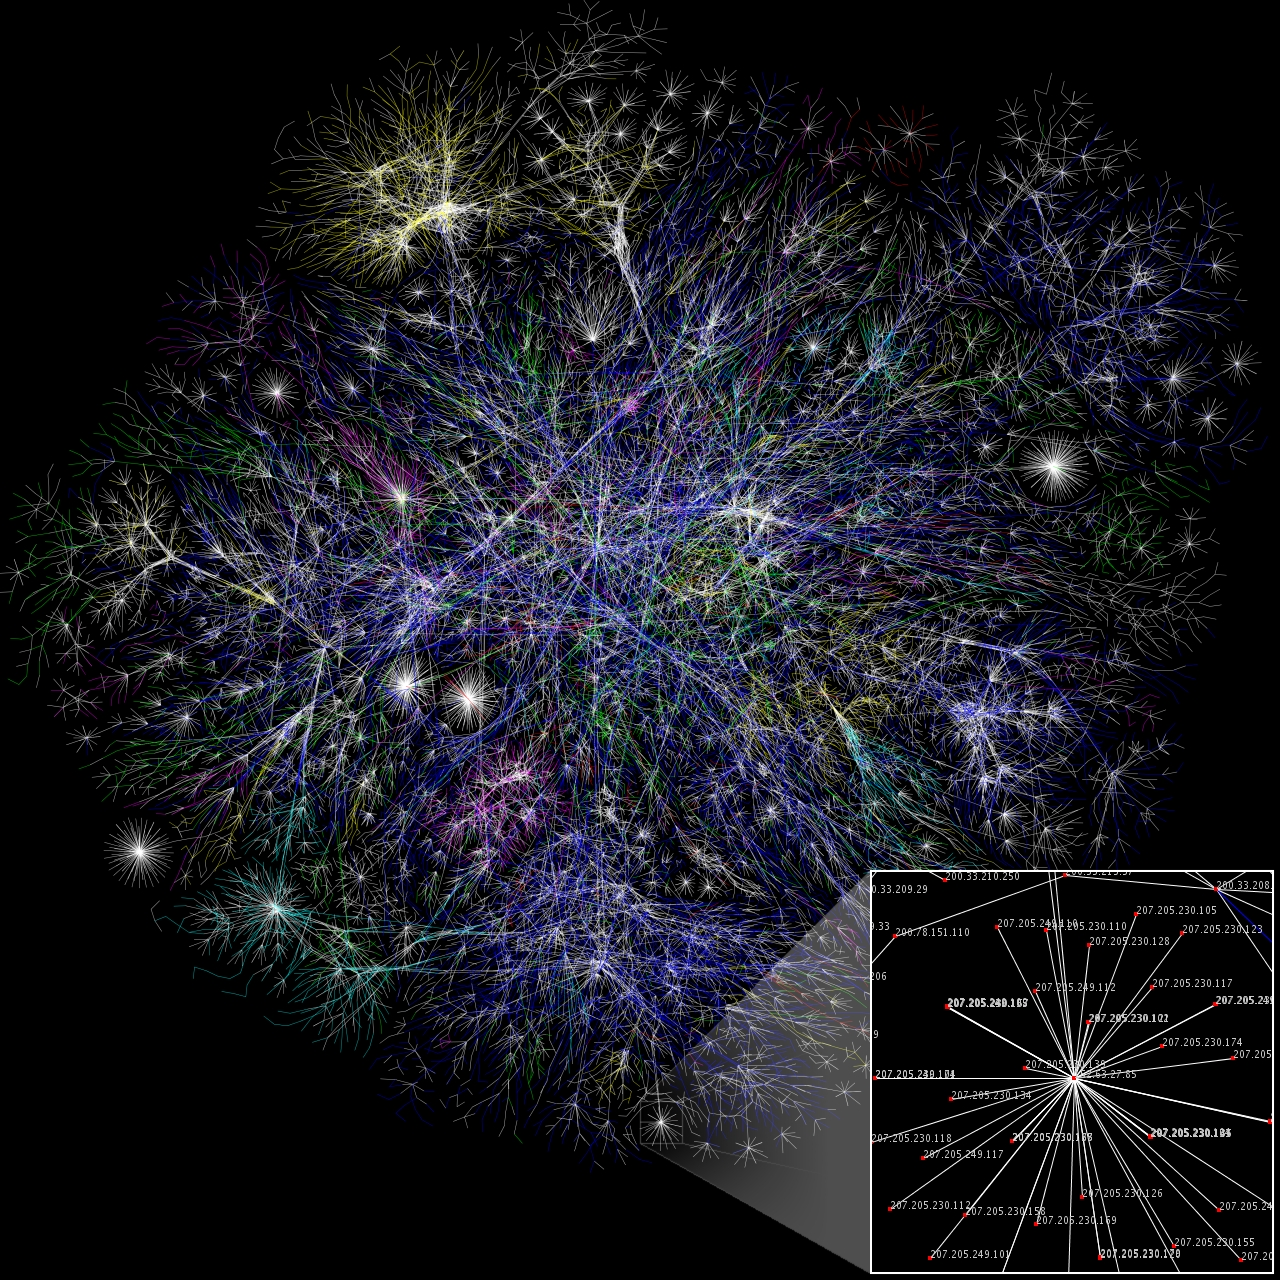
\includegraphics[width=\textwidth]{internet}
\end{columns}
\end{frame}


\begin{frame}{Hugbúnaðarhönnun}
\begin{itemize}
 \item Getum notað net til að hjálpa okkur við hönnun stórra forritunarkerfa
 \item Táknum forritseiningar (klasa, ``módúla'') með hnútum, setjum örvalegg þeirra á milli sé ein þeirra háð annarri
 \item Látum net tákna forkröfur í forriti sem keyra á með samhliða vinnslu
 \begin{itemize}
  \item Táknum búta forrits með hnútum, setjum örvalegg frá forritsbútum sem þurfa að hafa meiri forgang til þeirra sem minni mega hafa
 \end{itemize}
\end{itemize}
\end{frame}

\begin{frame}{Pakkakerfi}
\url{https://anvaka.github.io/pm/}
\end{frame}

\begin{frame}{Samgöngur og innviðir}
\begin{itemize}
 \item Getum táknað færslur alls kyns hluta og fyrirbrigða með netum
 \begin{itemize}
  \item Vegakerfi eða flugsamgöngur
  \begin{itemize}
   \item Táknum gatnamót með hnútum og vegi með leggjum 
   \item Táknum flugvelli með hnútum og flugleiðir með leggjum
  \end{itemize}
  \item Rafmagnsdreifikerfi eða vatnsdreifikerfi
  \begin{itemize}
   \item Táknum rafstöðvar með hnútum og rafmagnslínur með leggjum
   \item Táknum dælustöðvar með hnútum og vatnspípur með leggjum
  \end{itemize}
 \end{itemize}
 \item Gætum endað með óstefnd, örvanet eða blönduð net
\end{itemize}
\end{frame}

\begin{frame}{Net í líffræði}
\begin{itemize}
 \item Netaframsetningar koma víða við í ýmsum undirgreinum líffræði
 \begin{itemize}
  \item ``Niche overlap graphs'' í vistfræði
  \begin{itemize}
   \item Táknum tegund með hnútum, tengjum með legg ef þær eru í samkeppni
  \end{itemize}
  \item Víxlverkunarnet próteina
  \begin{itemize}
   \item Prótein hafa áhrif hvert á annað, táknum prótein með hnútum og táknum víxlverkanir með leggjum
  \end{itemize}
  \item Flæðinet fyrir efnaskipti í lífverum
  \begin{itemize}
   \item Táknum efnasambönd með hnútum og efnahvörf með örvaleggjum
   \item Námskeið við HÍ: Inngangur að kerfislíffræði
  \end{itemize}
 \end{itemize}
\end{itemize}
\end{frame}

\section{Hugtök sem tengjast netum}

\begin{frame}{Hugtök}
\begin{itemize}
 \item Tveir hnútar $u$ og $v$ eru aðlægir (e. \emph{adjacent}) í óstefndu neti $G$ ef bæði $u$ og $v$ koma fyrir í skilgreiningu einhvers leggs í $G$
 \item Nágrannar hnúts $v$ eru þeir hnútar sem eru aðlægir $v$
 \begin{itemize}
  \item Mengi nágranna hnútsins $v$ er táknað með $N(v)$
 \end{itemize}
 \item Stig (e. \emph{degree}) hnúts $v$ í óstefndu neti er fjöldi hnúta sem eru aðlægir $v$
 \begin{itemize}
  \item Lykkja á hnút ``telur tvöfalt'', hækkar stig hnútsins um 2
  \item Stig hnúts $v$ er táknað með $\deg(v)$
 \end{itemize}
\end{itemize}
\end{frame}

\begin{frame}{Handabandssetningin}
\begin{tcolorbox}[title=Handabandssetningin]
Látum $G = (V, E)$ vera óstefnt net með $m$ leggjum. Þá er
\[
 2m = \sum_{v \in V} \deg(v)
\]
\end{tcolorbox}
Handabandssetningin (e. \emph{the handshake theorem}) á við um fjölnet og net með lykkjum.
\end{frame}

\begin{frame}{Næst}
(Fleiri) hugtök í netafræði (10.2) og framsetning á netum (10.3)
\end{frame}


\end{document}
